\section{Experimental Results and Discussions}
This section presents experimental results. We implemented \mrtnet using PyTorch. 

\subsection{Shape classification} To demonstrate the effectiveness of the multiresolution encoder, we trained a baseline model that follows the same classification model but replacing multiresolution convolutions with single-scale 1D convolutions. Also, we apply the same test-time data augmentation and compute the test-time average as described in the Section~\ref{mrt:method}. %

\begin{table}[t]
    \begin{minipage}{0.5\linewidth}    
    \centering
    \begin{tabular}{p{4cm}>{\centering\arraybackslash}p{1.2cm}}
        \toprule
        Method & Accuracy\\
        \midrule
        \multicolumn{2}{l}{\textit{View-based methods}}  \\
        MVCNN~\cite{mvcnn}              &  90.1   \\
        MVCNN-MultiRes~\cite{qi2016volumetric}     &  91.4    \\
        \midrule
        \multicolumn{2}{l}{\textit{Point-based methods (w/o normals)}}   \\
        KDNet (1K pts)~\cite{Klokov_2017_ICCV}  & 90.6 \\
        PointNet (1K pts)~\cite{pointnet}   & 89.2 \\
        PointNet++ (1K pts)~\cite{pointnet2} &  90.7 \\
        MRTNet (1K pts)  & \textbf{91.2} \\
        MRTNet (4K pts)& \textbf{91.7} \\
        KDNet (32K pts)~\cite{Klokov_2017_ICCV}     & \textbf{91.8} \\
        \midrule
        \multicolumn{2}{l}{\textit{Point-based methods (with normals)}}   \\
        PointNet++ (5K pts)~\cite{pointnet2} &  91.9\\
        \midrule
        \multicolumn{2}{l}{\textit{Voxel-based methods}}   \\
        OctNet~\cite{Riegler2017CVPR}       & 86.5 \\
        O-CNN~\cite{ocnn}   & 90.6\\
        \midrule
   \end{tabular}
   \caption*{\small (a) \textbf{Comparisons with previous work}. Among point-based methods that use $xyz$ data only, ours is the best in the 1K points group; and our 4K result is comparable with KDNet at 32K points.}
   \end{minipage}
   \begin{minipage}{0.5\linewidth}
   \centering
    \begin{tabular}{p{4.0cm}>{\centering\arraybackslash}p{1.2cm}}
        \toprule
        Method & Accuracy\\
        \midrule
        Full model (MRTNet, 4K pts) & 91.7 \\
        Filters/4 & 91.7 \\
        Single res. & 89.3 \\
        Single res., no aug. (kd-tree) & 86.2 \\
        Single res., no aug. (rp-tree) & 87.4\\
        \midrule
        \end{tabular}
        \caption*{\small (b) \textbf{\mrtnet ablation studies}. Filters/4 reduces the number of filters in each layer by 4. The last three rows are the single resolution model.}

    \begin{tabular}{p{4.0cm}>{\centering\arraybackslash}p{1.2cm}}
        \midrule
        Method & Accuracy\\
        \midrule
        SPH~\cite{Kazhdan:2003} & 68.2 \\
        LFD~\cite{Chen03} & 75.5 \\
        T-L Network\cite{Girdhar16} & 74.4 \\
        VConv-DAE \cite{Sharma2016} & 75.5 \\
        3D-GAN~\cite{3dgan} & 83.3 \\
        MRTNet-VAE (Ours) & \textbf{86.4} \\
        \midrule
        \caption*{\small (c) \textbf{Unsupervised representation learning}. Section~\ref{sec:exp_gen}.}
        \end{tabular}
   \end{minipage}
    \caption{Instance classification accuracy on the ModelNet40 dataset.} \label{tab:class}
    \vspace{-18pt}
\end{table}

Classification benchmark results are in Table~\ref{tab:class}(a). 
As shown in the table, \mrtnet achieves the best results among all \textbf{point-based} methods that use $xyz$ data only. In particular, ours is the best in the 1K points group. We also experimented with sampling shapes using 4K points, and the result is comparable with KDNet at 32K points -- in this case, KDNet uses 8$\times$ more points (hence 8$\times$ more memory) than ours, and is only $0.1\%$ better. PointNet++~\cite{pointnet2} with 5K points and normals is $0.2\%$ better than ours.

\setlength{\intextsep}{0pt}%
\setlength{\columnsep}{0pt}%
\begin{wrapfigure}{r}{0.35\linewidth} 
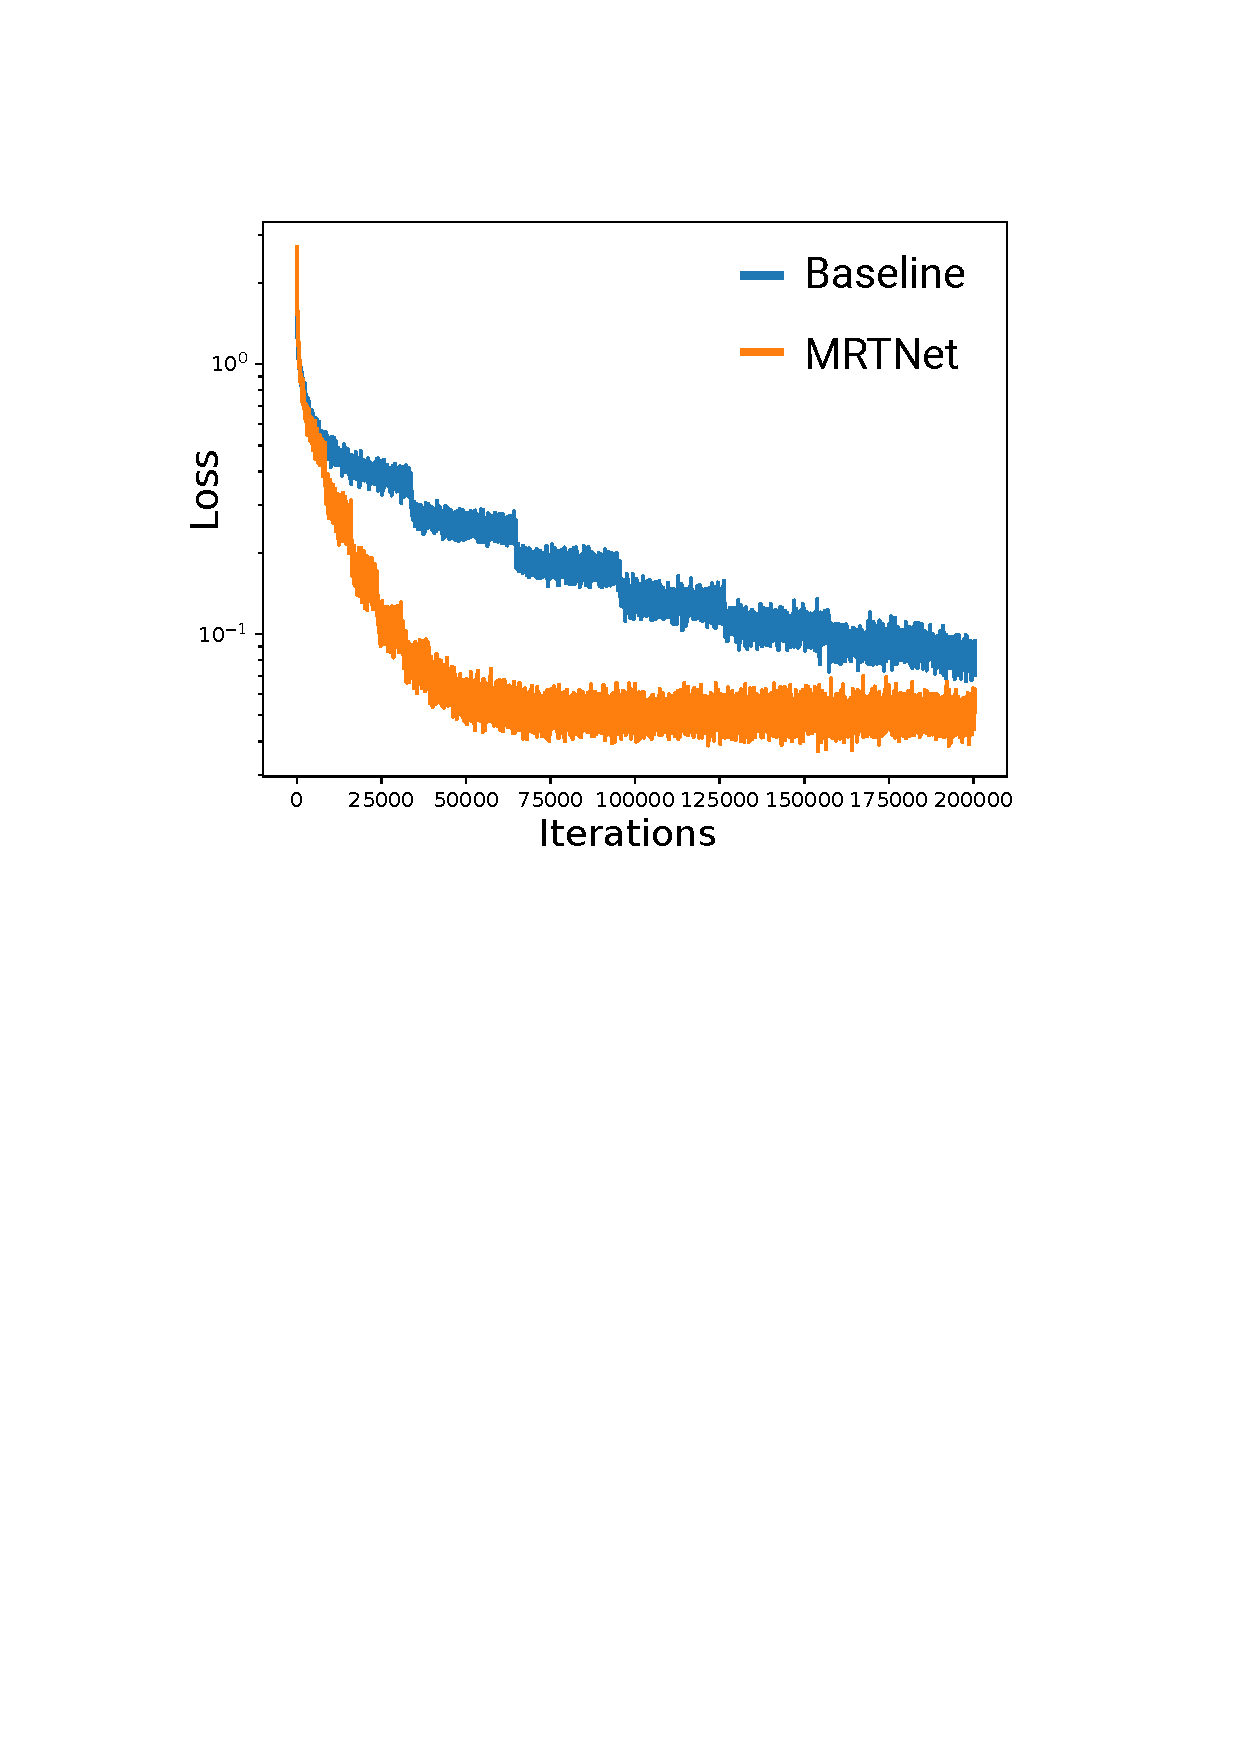
\includegraphics[width=1.0\linewidth]{MRTNet/imgs/convergence_loss.pdf}
\vspace{-20pt}
\caption{\small Cross entropy decay \label{fig:convergence}}
\end{wrapfigure} 
Table~\ref{tab:class}(b) shows ablation study results with variants of our approach.
Particularly, the multiresolution version is more than $2\%$ better than the baseline model (i.e. single resolution), 
while using the same number of parameters (the Filters/4 version). 
Besides, \mrtnet converges must faster than the baseline model, as we can see in the cross entropy loss decay plots in Figure~\ref{fig:convergence}. 
This shows that the multiresolution architecture leads to higher quality/accuracy and is memory efficient. 

Our single resolution baseline is akin to KDNet except it doesn't condition the convolutions on the splitting axes.
It results in $1.3\%$ less classification accuracy compared to KDNet (1K pts). This suggests that conditioning on the splitting axes during convolutions improves the accuracy.
However, this comes at the cost of extra book keeping and at least three times more parameters.
\mrtnet achieves greater benefits with lesser overhead.
Similar to the KDNet, our methods also benefit from data augmentation and can be used with both kd-trees and rp-trees.






\begin{table}[t]
\scriptsize
\centering
\begin{tabular}{c||c|c|c|c|c|c}
\hline
\multicolumn{1}{c||}{\multirow{2}{*}{\bf Category}} & \multicolumn{3}{c|}{3D-R2N2~\cite{choy20163d}} & Fan et al.~\cite{fan2016point} & Lin et al.~\cite{lin2018learning} & \mrtnet \\
& 1 view    & 3 views & 5 views & (1 view) & (1 view) & (1 view) \\ \hline
airplane & 3.207 / 2.879 & 2.521 / 2.468 & 2.399 / 2.391 & 1.301 / 1.488 & 1.294 / 1.541 & {\bf 0.976} / {\bf 0.920}\\
bench & 3.350 / 3.697 & 2.465 / 2.746 & 2.323 / 2.603 & 1.814 / 1.983 & 1.757 / 1.487 & {\bf 1.438} / {\bf 1.326}\\
cabinet & 1.636 / 2.817 & 1.445 / 2.626 & {\bf 1.420} / 2.619 & 2.463 / 2.444 & 1.814 / {\bf 1.072} & 1.774 / 1.602\\
car & 1.808 / 3.238 & 1.685 / 3.151 & 1.664 / 3.146 & 1.800 / 2.053 & 1.446 / {\bf 1.061} & {\bf 1.395} / 1.303\\
chair & 2.759 / 4.207 & 1.960 / 3.238 & 1.854 / 3.080 & 1.887 / 2.355 & 1.886 / 2.041 & {\bf 1.650} / {\bf 1.603}\\
display & 3.235 / 4.283 & 2.262 / 3.151 & 2.088 / 2.953 & 1.919 / 2.334 & 2.142 / {\bf 1.440} & {\bf 1.815} / 1.901\\
lamp & 8.400 / 9.722 & 6.001 / 7.755 & 5.698 / 7.331 & 2.347 / 2.212 & 2.635 / 4.459 & {\bf 1.944} / {\bf 2.089}\\
speaker & 2.652 / 4.335 & 2.577 / 4.302 & 2.487 / 4.203 & 3.215 / 2.788 & 2.371 / {\bf 1.706} & {\bf 2.165} / 2.121\\
rifle & 4.798 / 2.996 & 4.307 / 2.546 & 4.193 / 2.447 & 1.316 / 1.358 & 1.289 / 1.510 & {\bf 1.029} / {\bf 1.028}\\
sofa & 2.725 / 3.628 & 2.371 / 3.252 & 2.306 / 3.196 & 2.592 / 2.784 & 1.917 / {\bf 1.423} & {\bf 1.768} / 1.756\\
table & 3.118 / 4.208 & 2.268 / 3.277 & 2.128 / 3.134 & 1.874 / 2.229 & 1.689 / 1.620 & {\bf 1.570} / {\bf 1.405}\\
telephone & 2.202 / 3.314 & 1.969 / 2.834 & 1.874 / 2.734 & 1.516 / 1.989 & 1.939 / {\bf 1.198} & {\bf 1.346} / 1.332\\
watercraft & 3.592 / 4.007 & 3.299 / 3.698 & 3.210 / 3.614 & 1.715 / 1.877 & 1.813 / 1.550 & {\bf 1.394} / {\bf 1.490}\\
\hline
 \bf mean& 3.345 / 4.102 & 2.702 / 3.465 & 2.588 / 3.342 & 1.982 / 2.146 & 1.846 / 1.701 & {\bf 1.559} / {\bf 1.529}\\
\hline
\end{tabular}
\caption{\label{table:multi} \small \textbf{Single-image shape inference results}. The training data consists of 13 categories of shapes provided by~\cite{choy20163d}.     The numbers shown are [pred$\to$GT / GT$\to$pred] errors, scaled by 100. The mean is computed across all 13 categories. Our \mrtnet produces 4K points for each shape.
}
\vspace{-12pt}
\end{table}

\begin{table}[t]
\centering
\begin{tabular}{|c|c|c|}
\hline
Fully Connected & Single Res. & MRTNet \\
1.824 / 2.297 & 1.708 / 1.831 & {\bf 1.559} / {\bf 1.529} \\
\hline
\end{tabular}
\caption{\small
\label{table:ablation}
\textbf{Ablation studies for the image to shape decoder.} The numbers shown are [pred$\to$GT / GT$\to$pred] errors, scaled by 100. 
The values are the mean computed across all 13 categories.}
\vspace{-24pt}
\end{table}

\subsection{Single-image shape inference} \label{sec:exp_shapeinfer} We compare our single-image shape inference results with volumetric~\cite{choy20163d}, view-based~\cite{lin2018learning} and point-based~\cite{fan2016point} approaches using the evaluation metric by~\cite{lin2018learning}. 
Given a source point cloud $\mathbf{x}$ and a target point cloud $\mathbf{y}$, we compute
the average euclidean distance from each point in $\mathbf{x}$ to its closest in $\mathbf{y}$.
We refer to this as pred$\to$GT (prediction to groundtruth) error. It indicates how dissimilar the predicted shape is from the ground-truth.
The GT$\to$pred error is computed similarly by swapping $\mathbf{x}$ and $\mathbf{y}$, and it measures coverage (i.e. how complete the ground-truth surface was covered by the prediction).
For the voxel based model~\cite{choy20163d}, we used the same procedure as~\cite{lin2018learning},
where point clouds are formed by creating one point in the center of each surface voxel.
Surface voxels are extracted by subtracting the prediction by
its eroded version and rescale them such that the tightest 3D bounding boxes of the prediction and
the ground-truth CAD models have the same volume.

\begin{figure*}[t]
\centering
\setlength{\tabcolsep}{0pt}
\begin{tabular}{ccc|ccc|ccc}
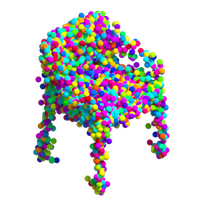
\includegraphics[width=.108\linewidth]{MRTNet/rendering/srfc_comparison/FCI2PC_all_vgg_True/cc25ba35b3f6e8d3d064b65ccd8977_mrt_v1.png} &
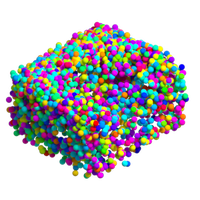
\includegraphics[width=.108\linewidth]{MRTNet/rendering/srfc_comparison/FCI2PC_all_vgg_True/cc2930e7ceb24691febad4f49b26ec_mrt_v1.png} &
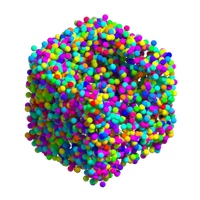
\includegraphics[width=.108\linewidth]{MRTNet/rendering/srfc_comparison/FCI2PC_all_vgg_True/cc03a89a98cd2660c423490470c47d_mrt_v1.png} &
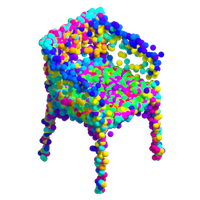
\includegraphics[width=.108\linewidth]{MRTNet/rendering/srfc_comparison/SRI2PC_all_vgg_True/cc25ba35b3f6e8d3d064b65ccd8977_mrt_v1.png} &
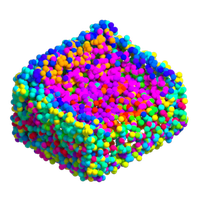
\includegraphics[width=.108\linewidth]{MRTNet/rendering/srfc_comparison/SRI2PC_all_vgg_True/cc2930e7ceb24691febad4f49b26ec_mrt_v1.png} &
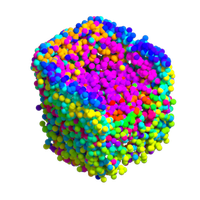
\includegraphics[width=.108\linewidth]{MRTNet/rendering/srfc_comparison/SRI2PC_all_vgg_True/cc03a89a98cd2660c423490470c47d_mrt_v1.png} &
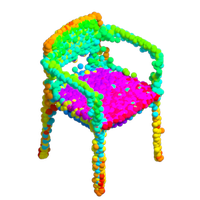
\includegraphics[width=.108\linewidth]{MRTNet/rendering/srfc_comparison/MRI2PC_all_vgg_True/cc25ba35b3f6e8d3d064b65ccd8977_mrt_v1.png} &
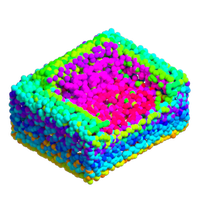
\includegraphics[width=.108\linewidth]{MRTNet/rendering/srfc_comparison/MRI2PC_all_vgg_True/cc2930e7ceb24691febad4f49b26ec_mrt_v1.png} &
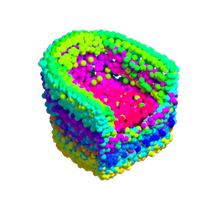
\includegraphics[width=.108\linewidth]{MRTNet/rendering/srfc_comparison/MRI2PC_all_vgg_True/cc03a89a98cd2660c423490470c47d_mrt_v1.png} \\

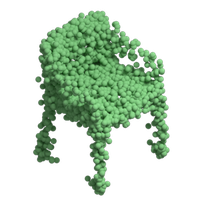
\includegraphics[width=.108\linewidth]{MRTNet/rendering/srfc_comparison/FCI2PC_all_vgg_True/cc25ba35b3f6e8d3d064b65ccd8977_mrt_green_v1.png} &
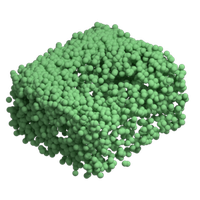
\includegraphics[width=.108\linewidth]{MRTNet/rendering/srfc_comparison/FCI2PC_all_vgg_True/cc2930e7ceb24691febad4f49b26ec_mrt_green_v1.png} &
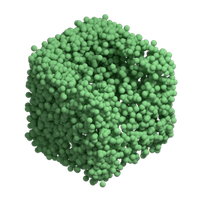
\includegraphics[width=.108\linewidth]{MRTNet/rendering/srfc_comparison/FCI2PC_all_vgg_True/cc03a89a98cd2660c423490470c47d_mrt_green_v1.png} &
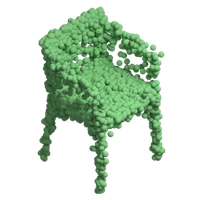
\includegraphics[width=.108\linewidth]{MRTNet/rendering/srfc_comparison/SRI2PC_all_vgg_True/cc25ba35b3f6e8d3d064b65ccd8977_mrt_green_v1.png} &
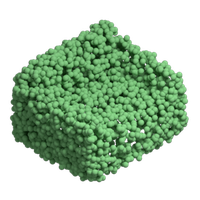
\includegraphics[width=.108\linewidth]{MRTNet/rendering/srfc_comparison/SRI2PC_all_vgg_True/cc2930e7ceb24691febad4f49b26ec_mrt_green_v1.png} &
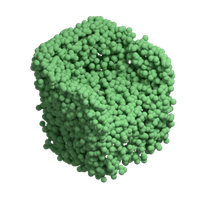
\includegraphics[width=.108\linewidth]{MRTNet/rendering/srfc_comparison/SRI2PC_all_vgg_True/cc03a89a98cd2660c423490470c47d_mrt_green_v1.png} &
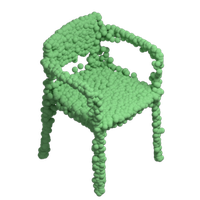
\includegraphics[width=.108\linewidth]{MRTNet/rendering/srfc_comparison/MRI2PC_all_vgg_True/cc25ba35b3f6e8d3d064b65ccd8977_mrt_green_v1.png} &
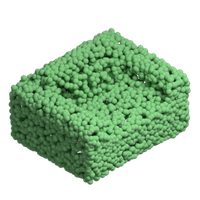
\includegraphics[width=.108\linewidth]{MRTNet/rendering/srfc_comparison/MRI2PC_all_vgg_True/cc2930e7ceb24691febad4f49b26ec_mrt_green_v1.png} &
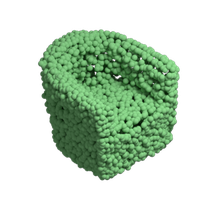
\includegraphics[width=.108\linewidth]{MRTNet/rendering/srfc_comparison/MRI2PC_all_vgg_True/cc03a89a98cd2660c423490470c47d_mrt_green_v1.png}
\end{tabular}
\vspace{-8pt}
    \caption{\label{fig:ablation-comp} 
    \small Shapes generated by 1) the fully connected baseline; 2) the single-resolution baseline; and 3) \mrtnet.
    Colors in the first row indicate the index of a point in the output point list.}
\vspace{-6pt}
\end{figure*}

\begin{figure*}[t]
\centering
\setlength{\tabcolsep}{0pt}
\begin{tabular}{c|cccccccc}
{\rotatebox[origin=lt]{90}{Input}} &
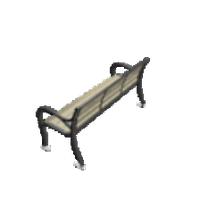
\includegraphics[width=.12\linewidth]{MRTNet/rendering/i2pc_comparison/c83b3192c338527a2056b4bd5d870b_alpha.png} &
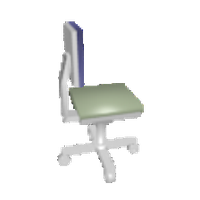
\includegraphics[width=.12\linewidth]{MRTNet/rendering/i2pc_comparison/cbe006da89cca7ffd6bab114dd47e3_alpha.png} &
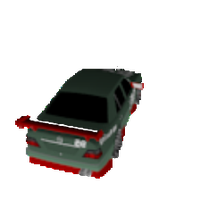
\includegraphics[width=.12\linewidth]{MRTNet/rendering/i2pc_comparison/cd24768b45ef5efcb1bb46d2556ba6_alpha.png} &
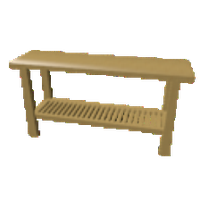
\includegraphics[width=.12\linewidth]{MRTNet/rendering/i2pc_comparison/cdee5ccae3613c507e1dc03b595bd3_alpha.png} &
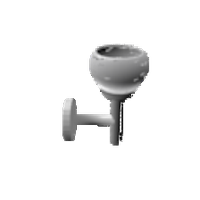
\includegraphics[width=.12\linewidth]{MRTNet/rendering/i2pc_comparison/d2d645ce6ad43434d42b9650f19dd4_alpha.png} &
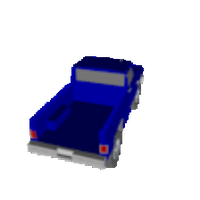
\includegraphics[width=.12\linewidth]{MRTNet/rendering/i2pc_comparison/ccc6b5ace9f5164d26068f53fe0ecf_alpha.png} &
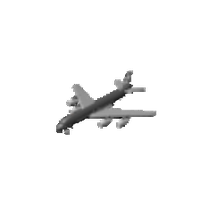
\includegraphics[width=.12\linewidth]{MRTNet/rendering/i2pc_comparison/d18592d9615b01bbbc0909d98a1ff2_alpha.png} &
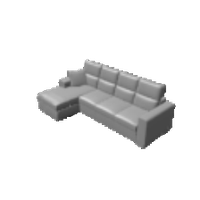
\includegraphics[width=.12\linewidth]{MRTNet/rendering/i2pc_comparison/cceaeed0d8cf5bdbca68d7e2f215cb_alpha.png} \\
\hline
{\rotatebox[origin=lt]{90}{G.T.}} &
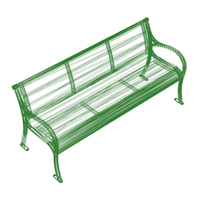
\includegraphics[width=.12\linewidth]{MRTNet/rendering/i2pc_comparison/gt/img1.png} &
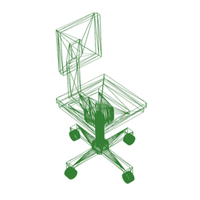
\includegraphics[width=.12\linewidth]{MRTNet/rendering/i2pc_comparison/gt/img2.png} &
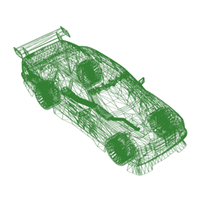
\includegraphics[width=.12\linewidth]{MRTNet/rendering/i2pc_comparison/gt/img3.png} &
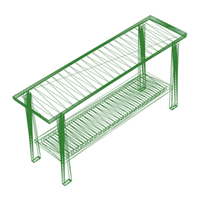
\includegraphics[width=.12\linewidth]{MRTNet/rendering/i2pc_comparison/gt/img4.png} &
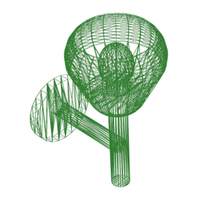
\includegraphics[width=.12\linewidth]{MRTNet/rendering/i2pc_comparison/gt/img5.png} &
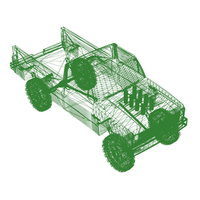
\includegraphics[width=.12\linewidth]{MRTNet/rendering/i2pc_comparison/gt/img6_alt.png} &
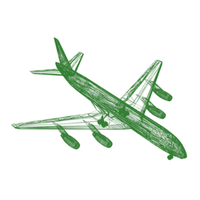
\includegraphics[width=.12\linewidth]{MRTNet/rendering/i2pc_comparison/gt/img7.png} &
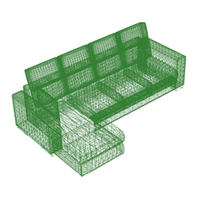
\includegraphics[width=.12\linewidth]{MRTNet/rendering/i2pc_comparison/gt/img8.png} \\
\hline
{\rotatebox[origin=lt]{90}{\mrtnet}} &
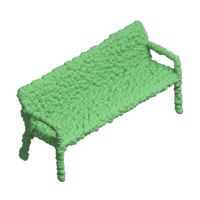
\includegraphics[width=.12\linewidth]{MRTNet/rendering/i2pc_comparison/c83b3192c338527a2056b4bd5d870b_mrt_v1.png} &
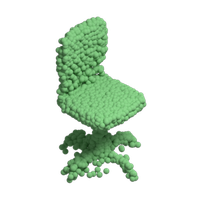
\includegraphics[width=.12\linewidth]{MRTNet/rendering/i2pc_comparison/cbe006da89cca7ffd6bab114dd47e3_mrt_v1.png} &
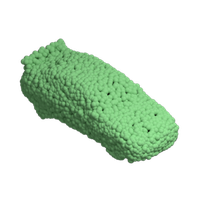
\includegraphics[width=.12\linewidth]{MRTNet/rendering/i2pc_comparison/cd24768b45ef5efcb1bb46d2556ba6_mrt_v1.png} &
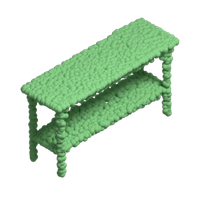
\includegraphics[width=.12\linewidth]{MRTNet/rendering/i2pc_comparison/cdee5ccae3613c507e1dc03b595bd3_mrt_v1.png} &
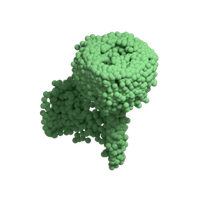
\includegraphics[width=.12\linewidth]{MRTNet/rendering/i2pc_comparison/d2d645ce6ad43434d42b9650f19dd4_mrt_v1.png} &
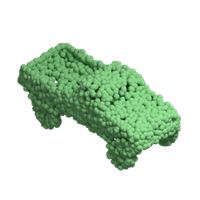
\includegraphics[width=.12\linewidth]{MRTNet/rendering/i2pc_comparison/ccc6b5ace9f5164d26068f53fe0ecf_mrt_v1.png} &
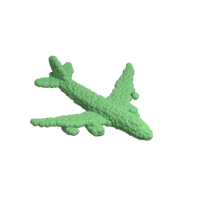
\includegraphics[width=.12\linewidth]{MRTNet/rendering/i2pc_comparison/d18592d9615b01bbbc0909d98a1ff2_mrt_v1.png} &
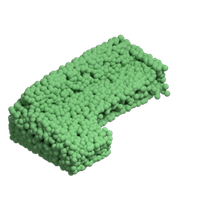
\includegraphics[width=.12\linewidth]{MRTNet/rendering/i2pc_comparison/cceaeed0d8cf5bdbca68d7e2f215cb_mrt_v1.png} \\
\hline
{\rotatebox[origin=lt]{90}{\small Fan~\cite{fan2016point}}} &
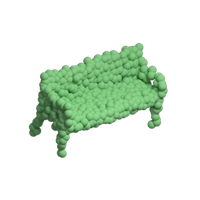
\includegraphics[width=.12\linewidth]{MRTNet/rendering/i2pc_comparison/c83b3192c338527a2056b4bd5d870b_alignedpsg_v1.png} &
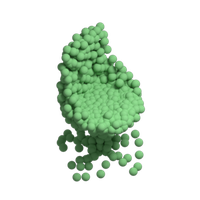
\includegraphics[width=.12\linewidth]{MRTNet/rendering/i2pc_comparison/cbe006da89cca7ffd6bab114dd47e3_alignedpsg_v1.png} &
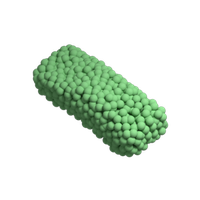
\includegraphics[width=.12\linewidth]{MRTNet/rendering/i2pc_comparison/cd24768b45ef5efcb1bb46d2556ba6_alignedpsg_v1.png} &
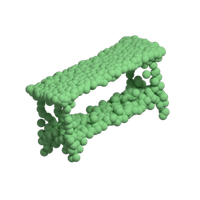
\includegraphics[width=.12\linewidth]{MRTNet/rendering/i2pc_comparison/cdee5ccae3613c507e1dc03b595bd3_alignedpsg_v1.png} &
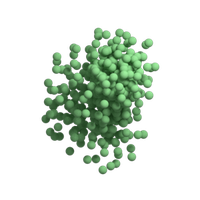
\includegraphics[width=.12\linewidth]{MRTNet/rendering/i2pc_comparison/d2d645ce6ad43434d42b9650f19dd4_alignedpsg_v1.png} &
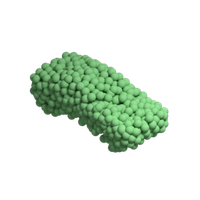
\includegraphics[width=.12\linewidth]{MRTNet/rendering/i2pc_comparison/ccc6b5ace9f5164d26068f53fe0ecf_alignedpsg_v1.png} &
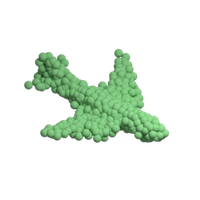
\includegraphics[width=.12\linewidth]{MRTNet/rendering/i2pc_comparison/d18592d9615b01bbbc0909d98a1ff2_alignedpsg_v1.png} &
\includegraphics[width=.12\linewidth]{MRTNet/rendering/i2pc_comparison/cceaeed0d8cf5bdbca68d7e2f215cb_alignedpsg_v1.png} \\
\hline
{\rotatebox[origin=lt]{90}{\small Choy~\cite{choy20163d}}} &
\includegraphics[width=.12\linewidth]{MRTNet/rendering/i2pc_comparison/c83b3192c338527a2056b4bd5d870b_r2n2_v1.png} &
\includegraphics[width=.12\linewidth]{MRTNet/rendering/i2pc_comparison/cbe006da89cca7ffd6bab114dd47e3_r2n2_v1.png} &
\includegraphics[width=.12\linewidth]{MRTNet/rendering/i2pc_comparison/cd24768b45ef5efcb1bb46d2556ba6_r2n2_v1.png} &
\includegraphics[width=.12\linewidth]{MRTNet/rendering/i2pc_comparison/cdee5ccae3613c507e1dc03b595bd3_r2n2_v1.png} &
\includegraphics[width=.12\linewidth]{MRTNet/rendering/i2pc_comparison/d2d645ce6ad43434d42b9650f19dd4_r2n2_v1.png} &
\includegraphics[width=.12\linewidth]{MRTNet/rendering/i2pc_comparison/ccc6b5ace9f5164d26068f53fe0ecf_r2n2_v1.png} &
\includegraphics[width=.12\linewidth]{MRTNet/rendering/i2pc_comparison/d18592d9615b01bbbc0909d98a1ff2_r2n2_v1.png} &
\includegraphics[width=.12\linewidth]{MRTNet/rendering/i2pc_comparison/cceaeed0d8cf5bdbca68d7e2f215cb_r2n2_v1.png} \\
\hline
\end{tabular}
\vspace{-8pt}
    \caption{\label{fig:inference-comp} 
    \small Qualitative results for single-image shape inference. From top to bottom: input images, ground truth 3D shapes, results of \mrtnet, Fan et al.~\cite{fan2016point}, and Choy et al.~\cite{choy20163d}.
    }
\vspace{-12pt}
\end{figure*}

Table~\ref{table:multi} shows our results. 
Our solution outperforms competing methods in 12 out of 13 categories on the pred$\to$GT error, and in
6 categories on GT$\to$pred error.
Note that we are consistently better than the point-based methods such as~\cite{fan2016point} in both metrics; 
and we are consistently better than~\cite{lin2018learning} in the pred$\to$GT metric.
Furthermore, our method wins by a considerable margin in terms of the mean per category on both metrics. 
It is important to highlight that the multi-view based method~\cite{lin2018learning} produces tens of thousands of points and many of them
are not in the right positions, which penalizes their pred$\to$GT metric, but that helps to improve their GT$\to$pred.
Moreover, as mentioned in~\cite{lin2018learning}, their method has difficulties capturing thin structures (e.g. lamps) whereas ours is able
to capture them relatively well.
For example, our GT$\to$pred error for the \textbf{lamp} category (which contains many thin geometric structures) is more than two times smaller than the error by~\cite{lin2018learning}, indicating that MRTNet is more successful at capturing thin structures in the shapes.

\para{Ablation studies.}
In order to quantify the effectiveness of the multiresolution decoder, we compared our method with two
different baselines: a fully connected decoder and a single-resolution decoder.
The fully connected decoder consists of 3 linear layers with 4096 hidden neurons, each layer followed by batch normalization 
and ReLU activation units.
On top of that, we add a final layer that outputs $4096\times3$ values corresponding to the final point cloud, followed
by a hyperbolic tangent activation function.
The single resolution decoder follows the same architecture of the MRT decoder but replacing multiresolution convolutions with single-scale 1D convolutions.
Results are shown in Table~\ref{table:ablation}.
Note that both baselines are quite competitive. 
The single-resolution decoder is comparable to the result of~\cite{lin2018learning}, while the fully connected one achieves similar mean errors to~\cite{fan2016point}.
Still, they fall noticeably behind \mrtnet.


\begin{figure*}[t]
\centering
\setlength{\tabcolsep}{0pt}
\begin{tabular}{cccccccc}
    
\includegraphics[width=.12\linewidth]{MRTNet/rendering/real_MRI2PC/out_0000.png} &
\includegraphics[width=.12\linewidth]{MRTNet/rendering/real_MRI2PC/tables/table8_mrt.png} &
\includegraphics[width=.12\linewidth]{MRTNet/rendering/real_MRI2PC/out_0002.png} &
\includegraphics[width=.12\linewidth]{MRTNet/rendering/real_MRI2PC/tables/table2_mrt.png} &
\includegraphics[width=.12\linewidth]{MRTNet/rendering/real_MRI2PC/out_0004.png} &
\includegraphics[width=.12\linewidth]{MRTNet/rendering/real_MRI2PC/tables/table3_mrt.png} &
\includegraphics[width=.12\linewidth]{MRTNet/rendering/real_MRI2PC/tables/table5_mrt.png} &
\includegraphics[width=.12\linewidth]{MRTNet/rendering/real_MRI2PC/out_0007.png} \\

\includegraphics[width=.12\linewidth]{MRTNet/rendering/real_MRI2PC/out_0000_v1.png} &
\includegraphics[width=.12\linewidth]{MRTNet/rendering/real_MRI2PC/tables/table8_mrt_v1.png} &
\includegraphics[width=.12\linewidth]{MRTNet/rendering/real_MRI2PC/out_0002_v1.png} &
\includegraphics[width=.12\linewidth]{MRTNet/rendering/real_MRI2PC/tables/table2_mrt_v1.png} &
\includegraphics[width=.12\linewidth]{MRTNet/rendering/real_MRI2PC/out_0004_v1.png} &
\includegraphics[width=.12\linewidth]{MRTNet/rendering/real_MRI2PC/tables/table3_mrt_v1.png} &
\includegraphics[width=.12\linewidth]{MRTNet/rendering/real_MRI2PC/tables/table5_mrt_v1.png} &
\includegraphics[width=.12\linewidth]{MRTNet/rendering/real_MRI2PC/out_0007_v1.png} \\

\includegraphics[width=.12\linewidth]{MRTNet/rendering/real_MRI2PC/out_0000_v0.png} &
\includegraphics[width=.12\linewidth]{MRTNet/rendering/real_MRI2PC/tables/table8_mrt_v0.png} &
\includegraphics[width=.12\linewidth]{MRTNet/rendering/real_MRI2PC/out_0002_v0.png} &
\includegraphics[width=.12\linewidth]{MRTNet/rendering/real_MRI2PC/tables/table2_mrt_v0.png} &
\includegraphics[width=.12\linewidth]{MRTNet/rendering/real_MRI2PC/out_0004_v0.png} &
\includegraphics[width=.12\linewidth]{MRTNet/rendering/real_MRI2PC/tables/table3_mrt_v0.png} &
\includegraphics[width=.12\linewidth]{MRTNet/rendering/real_MRI2PC/tables/table5_mrt_v0.png} &
\includegraphics[width=.12\linewidth]{MRTNet/rendering/real_MRI2PC/out_0007_v0.png} \\

\hline

\includegraphics[width=.12\linewidth]{MRTNet/rendering/playdoh_shapes/plane3_mrt.png} &
\includegraphics[width=.12\linewidth]{MRTNet/rendering/playdoh_shapes/car8_clipped_rev_1_mrt.png} &
\includegraphics[width=.12\linewidth]{MRTNet/rendering/playdoh_shapes/5701697_clipped_rev_1_mrt.png} &
\includegraphics[width=.12\linewidth]{MRTNet/rendering/playdoh_shapes/cara_clipped_rev_1_mrt.png} &
\includegraphics[width=.12\linewidth]{MRTNet/rendering/playdoh_shapes/ship9_mrt.png} &
\includegraphics[width=.12\linewidth]{MRTNet/rendering/playdoh_shapes/ship3_mrt.png} &
\includegraphics[width=.12\linewidth]{MRTNet/rendering/playdoh_shapes/Play-Doh-Sofa_clipped_rev_1_mrt.png} &
\includegraphics[width=.12\linewidth]{MRTNet/rendering/playdoh_shapes/plane2_mrt.png} \\

\includegraphics[width=.12\linewidth]{MRTNet/rendering/playdoh_shapes/plane3_mrt_v0.png} &
\includegraphics[width=.12\linewidth]{MRTNet/rendering/playdoh_shapes/car8_clipped_rev_1_mrt_v0.png} &
\includegraphics[width=.12\linewidth]{MRTNet/rendering/playdoh_shapes/5701697_clipped_rev_1_mrt_v0.png} &
\includegraphics[width=.12\linewidth]{MRTNet/rendering/playdoh_shapes/cara_clipped_rev_1_mrt_v0.png} &
\includegraphics[width=.12\linewidth]{MRTNet/rendering/playdoh_shapes/ship9_mrt_v0.png} &
\includegraphics[width=.12\linewidth]{MRTNet/rendering/playdoh_shapes/ship3_mrt_v0.png} &
\includegraphics[width=.12\linewidth]{MRTNet/rendering/playdoh_shapes/Play-Doh-Sofa_clipped_rev_1_mrt_v0.png} &
\includegraphics[width=.12\linewidth]{MRTNet/rendering/playdoh_shapes/plane2_mrt_v0.png} \\

\includegraphics[width=.12\linewidth]{MRTNet/rendering/playdoh_shapes/plane3_mrt_v1.png} &
\includegraphics[width=.12\linewidth]{MRTNet/rendering/playdoh_shapes/car8_clipped_rev_1_mrt_v1.png} &
\includegraphics[width=.12\linewidth]{MRTNet/rendering/playdoh_shapes/5701697_clipped_rev_1_mrt_v1.png} &
\includegraphics[width=.12\linewidth]{MRTNet/rendering/playdoh_shapes/cara_clipped_rev_1_mrt_v1.png} &
\includegraphics[width=.12\linewidth]{MRTNet/rendering/playdoh_shapes/ship9_mrt_v1.png} &
\includegraphics[width=.12\linewidth]{MRTNet/rendering/playdoh_shapes/ship3_mrt_v1.png} &
\includegraphics[width=.12\linewidth]{MRTNet/rendering/playdoh_shapes/Play-Doh-Sofa_clipped_rev_1_mrt_v1.png} &
\includegraphics[width=.12\linewidth]{MRTNet/rendering/playdoh_shapes/plane2_mrt_v1.png} \\

\end{tabular}
\vspace{-8pt}
    \caption{\label{fig:real} 
    \small Shapes generated by applying \mrtnet on Inernet photos of furnitures and toys. \mrtnet is trained on the 13 categories of ShapeNet database (Table~\ref{table:multi}) . Note how the network is capable of generating detailed shapes from real photos, even though it is trained only on rendered images using simple shading models. For each output shape we show two different views.
    }
\vspace{-18pt}
\end{figure*}

In Figure~\ref{fig:ablation-comp} we visualize the structures of the output point clouds generated by the three methods.
The point clouds generated by MRTNet
present strong spatial coherence: points that are spatially nearby in 3D are also likely to be nearby in the 1D list.
This coherence is present to some degree in the single-resolution outputs (note the dark blue points in the chair's arms), but is almost completely absent in the results by the fully connected decoder. This is expected,
since fully connected layers do not leverage the spatial correlation of their inputs.
Operating at multiple scales enables MRTNet to enforce a stronger spatial coherence, allowing it to more efficiently synthesize detailed point clouds with coherent geometric structures.

\para{Qualitative results.} In Figure~\ref{fig:inference-comp} we present qualitative results of our method and comparisons to two prior works. 
The input images have 3 color channels and dimensions $224\times224$. 
In Figure~\ref{fig:real} we show results of our method applied on photographs downloaded from the Internet. 
To apply our method, we manually removed the background from the photos using~\cite{clipmagic}, which generally took less than half a minute per photo. 
As seen from the results, MRTNet is able to capture the structure and interesting geometric details of the objects (e.g. wheels of the office chairs), 
even though the input images are considerably different from the rendered ones used in training.


\begin{figure*}[t]
\centering
\setlength{\tabcolsep}{0pt}
\begin{tabular}{ccccccccc}
{\rotatebox[origin=lt]{90}{\mrtnet}} &
\includegraphics[width=.12\linewidth]{MRTNet/rendering/selected/mr_chairs/pc_0001.png} &
\includegraphics[width=.12\linewidth]{MRTNet/rendering/selected/mr_chairs/pc_0006.png} &
\includegraphics[width=.12\linewidth]{MRTNet/rendering/selected/mr_chairs/pc_0007.png} &
\includegraphics[width=.12\linewidth]{MRTNet/rendering/selected/mr_chairs/pc_0014.png} &
\includegraphics[width=.12\linewidth]{MRTNet/rendering/selected/mr_chairs/pc_0027.png} &
\includegraphics[width=.12\linewidth]{MRTNet/rendering/selected/mr_chairs/pc_0036.png} &
\includegraphics[width=.12\linewidth]{MRTNet/rendering/selected/mr_chairs/pc_0045.png} &
\includegraphics[width=.12\linewidth]{MRTNet/rendering/selected/mr_chairs/pc_0063.png} \\
{\rotatebox[origin=lt]{90}{Baseline}} &
\includegraphics[width=.12\linewidth]{MRTNet/rendering/selected/ae_chairs/pc_0000.png} &
\includegraphics[width=.12\linewidth]{MRTNet/rendering/selected/ae_chairs/pc_0001.png} &
\includegraphics[width=.12\linewidth]{MRTNet/rendering/selected/ae_chairs/pc_0003.png} &
\includegraphics[width=.12\linewidth]{MRTNet/rendering/selected/ae_chairs/pc_0004.png} &
\includegraphics[width=.12\linewidth]{MRTNet/rendering/selected/ae_chairs/pc_0006.png} &
\includegraphics[width=.12\linewidth]{MRTNet/rendering/selected/ae_chairs/pc_0007.png} &
\includegraphics[width=.12\linewidth]{MRTNet/rendering/selected/ae_chairs/pc_0008.png} &
\includegraphics[width=.12\linewidth]{MRTNet/rendering/selected/ae_chairs/pc_0009.png} \\
\end{tabular}
\vspace{-8pt}
    \caption{\label{fig:chairs-comp} 
    \small Qualitative comparisons of \mrvae with a single-resolution baseline model. Results are generated by randomly sampling the encoding $\encoding$. 
    \mrvae is able to preserve shape details much better than the baseline model, and produces less noisy outputs.}
\vspace{-6pt}
\end{figure*}
\begin{figure*}[t]
\centering
\setlength{\tabcolsep}{0pt}
\begin{tabular}{cccccccccccccccc}
\includegraphics[width=.1\linewidth]{MRTNet/rendering/selected/rec_shapenet/pc_0000.png} &
\includegraphics[width=.1\linewidth]{MRTNet/rendering/selected/rec_shapenet/pc_0002.png} &
\includegraphics[width=.1\linewidth]{MRTNet/rendering/selected/rec_shapenet/pc_0003.png} &
\includegraphics[width=.1\linewidth]{MRTNet/rendering/selected/rec_shapenet/pc_0004.png} &
\includegraphics[width=.1\linewidth]{MRTNet/rendering/selected/rec_shapenet/pc_0008.png} &
\includegraphics[width=.1\linewidth]{MRTNet/rendering/selected/rec_shapenet/pc_0011.png} &
\includegraphics[width=.1\linewidth]{MRTNet/rendering/selected/rec_shapenet/pc_0013.png} &
\includegraphics[width=.1\linewidth]{MRTNet/rendering/selected/rec_shapenet/pc_0015.png} &
\includegraphics[width=.1\linewidth]{MRTNet/rendering/selected/rec_shapenet/pc_0016.png} &
\includegraphics[width=.1\linewidth]{MRTNet/rendering/selected/rec_shapenet/pc_0018.png} \\
\includegraphics[width=.1\linewidth]{MRTNet/rendering/selected/rec_shapenet/pc_0025.png} &
\includegraphics[width=.1\linewidth]{MRTNet/rendering/selected/rec_shapenet/pc_0026.png} &
\includegraphics[width=.1\linewidth]{MRTNet/rendering/selected/rec_shapenet/pc_0027.png} &
\includegraphics[width=.1\linewidth]{MRTNet/rendering/selected/rec_shapenet/pc_0033.png} &
\includegraphics[width=.1\linewidth]{MRTNet/rendering/selected/rec_shapenet/pc_0035.png} &
\includegraphics[width=.1\linewidth]{MRTNet/rendering/selected/rec_shapenet/pc_0037.png} &
\includegraphics[width=.1\linewidth]{MRTNet/rendering/selected/rec_shapenet/pc_0042.png} &
\includegraphics[width=.1\linewidth]{MRTNet/rendering/selected/rec_shapenet/pc_0044.png} &
\includegraphics[width=.1\linewidth]{MRTNet/rendering/selected/rec_shapenet/pc_0048.png} &
\includegraphics[width=.1\linewidth]{MRTNet/rendering/selected/rec_shapenet/pc_0054.png}
\end{tabular}
\vspace{-12pt}
    \caption{\label{mrt:gallery} 
    \small Test set shapes reconstructed by \mrvae trained on all categories of ShapeNet (using 80\%/20\% training/test split). \mrvae is able to reconstruct high-quality diverse shapes.}
    \vspace{-8pt}
\end{figure*}

\subsection{Unsupervised Learning of Point Clouds} \label{sec:exp_gen}
For unsupervised learning of point clouds, we train our \mrvae using the ShapeNet dataset~\cite{chang2015shapenet}. 
By default we compute $N=4K$ points for each shape using Poisson Disk sampling~\cite{Bowers:2010:PPD} to evenly disperse the points. 
Each point set is then spatially sorted using a \kdtree. 
Here we use the vanilla \kdtree where the splitting axes alternate between $x$, $y$, $z$ at each level of the tree. 
The spatially sorted points are used as input to train the \mrvae network (Section~\ref{mrt:method}). 
Similar to before, we also train a baseline model that follows the same network but replacing multiresolution convolutions with single-scale 1D convolutions
in both encoder and decoder. 
As Figure~\ref{fig:chairs-comp} shows, the shapes generated by the \mrvae trained on chairs are of considerably higher quality than those generated by the baseline model. 

We also performed multiple-category shape generation by training \mrvae on $80\%$ of the objects from ShapeNet dataset. 
The remaining models belong to our test split. 
Reconstructions of objects in the test split are included in Figure~\ref{mrt:gallery}. 
Even when trained with a greater variety of shapes, the \mrvae is able to reconstruct high quality shapes from its embedding. 
This demonstrates that \mrvae is suitable for various inference tasks such as shape completion or point cloud reconstructions.

\para{Point ordering in the generated shapes.} 
A useful way to analyze shape generation is to see if the generated points have any consistent ordering across different shapes. 
This is an interesting question because as described previously, our \mrvae is trained using Chamfer Distance, 
a metric that's invariant to permutations of points. 
While the input to the network is all spatially sorted, the output is not restricted to any particular order and can in theory assume any arbitrary order. 
In practice, similar to the image-to-shape model, we observe that there is a consistent ordering of points in the generated shapes, as shown in Figure~\ref{fig:corresp}. 
Specifically, we picked three index ranges from one example chair, one at the top, one on the side, and one close to the bottom, 
then we color coded points in each shape that fall into these three index ranges. 
In the figure we can see clearly that they fall into approximately corresponding regions on each chair shape.

\begin{figure*}[t]
\centering
\setlength{\tabcolsep}{0pt}
\begin{tabular}{cccccccccccc}
\includegraphics[width=.083\linewidth]{MRTNet/rendering/selected/corresp/m1.png} &
\includegraphics[width=.083\linewidth]{MRTNet/rendering/selected/corresp/m2.png} &
\includegraphics[width=.083\linewidth]{MRTNet/rendering/selected/corresp/m3.png} &
\includegraphics[width=.083\linewidth]{MRTNet/rendering/selected/corresp/m4.png} &
\includegraphics[width=.083\linewidth]{MRTNet/rendering/selected/corresp/m5.png} &
\includegraphics[width=.083\linewidth]{MRTNet/rendering/selected/corresp/m6.png} &
\includegraphics[width=.083\linewidth]{MRTNet/rendering/selected/corresp/m7.png} &
\includegraphics[width=.083\linewidth]{MRTNet/rendering/selected/corresp/m8.png} &
\includegraphics[width=.083\linewidth]{MRTNet/rendering/selected/corresp/m9.png} &
\includegraphics[width=.083\linewidth]{MRTNet/rendering/selected/corresp/m10.png} &
\includegraphics[width=.083\linewidth]{MRTNet/rendering/selected/corresp/m11.png} &
\includegraphics[width=.083\linewidth]{MRTNet/rendering/selected/corresp/m12.png} 
\end{tabular}
\vspace{-8pt}
    \caption{\small \label{fig:corresp} Point correspondences among different shapes generated by \mrvae. 
	We picked three index ranges (indicated by three colors) from one example chair, and then color coded points in every shape that fall into these three ranges. 
	The images clearly show that the network learned to generate shapes with consistent point ordering.
    }
    \vspace{-4pt}
\end{figure*}

\begin{figure*}[t]
\centering
\setlength{\tabcolsep}{0pt}
\begin{tabular}{cccccccccc}
\includegraphics[width=.1\linewidth]{MRTNet/rendering/selected/interp1/pc_0000.png} &
\includegraphics[width=.1\linewidth]{MRTNet/rendering/selected/interp1/pc_0004.png} &
\includegraphics[width=.1\linewidth]{MRTNet/rendering/selected/interp1/pc_0006.png} &
\includegraphics[width=.1\linewidth]{MRTNet/rendering/selected/interp1/pc_0008.png} &
\includegraphics[width=.1\linewidth]{MRTNet/rendering/selected/interp1/pc_0009.png} &
\includegraphics[width=.1\linewidth]{MRTNet/rendering/selected/interp1/pc_0049.png} &
\includegraphics[width=.1\linewidth]{MRTNet/rendering/selected/interp1/pc_0058.png} &
\includegraphics[width=.1\linewidth]{MRTNet/rendering/selected/interp1/pc_0070.png} &
\includegraphics[width=.1\linewidth]{MRTNet/rendering/selected/interp1/pc_0080.png} &
\includegraphics[width=.1\linewidth]{MRTNet/rendering/selected/interp1/pc_0099.png} \\
\includegraphics[width=.1\linewidth]{MRTNet/rendering/selected/interp2/pc_0000.png} &
\includegraphics[width=.1\linewidth]{MRTNet/rendering/selected/interp2/pc_0004.png} &
\includegraphics[width=.1\linewidth]{MRTNet/rendering/selected/interp2/pc_0007.png} &
\includegraphics[width=.1\linewidth]{MRTNet/rendering/selected/interp2/pc_0009.png} &
\includegraphics[width=.1\linewidth]{MRTNet/rendering/selected/interp2/pc_0010.png} &
\includegraphics[width=.1\linewidth]{MRTNet/rendering/selected/interp2/pc_0011.png} &
\includegraphics[width=.1\linewidth]{MRTNet/rendering/selected/interp2/pc_0012.png} &
\includegraphics[width=.1\linewidth]{MRTNet/rendering/selected/interp2/pc_0014.png} &
\includegraphics[width=.1\linewidth]{MRTNet/rendering/selected/interp2/pc_0017.png} &
\includegraphics[width=.1\linewidth]{MRTNet/rendering/selected/interp2/pc_0019.png} 
\end{tabular}
    \vspace{-8pt}
    \caption{\small \label{mrt:interp} Shape interpolation results. For each example, we obtain the encodings $\encoding$ of the starting shape and ending shape, then linearly interpolate the encodings and use the decoder to generate output shapes from the interpolated $\encoding$. Results show plausible interpolated shapes.
    }
    \vspace{-16pt}   
\end{figure*}

\para{Shape interpolation.} Another common test is shape interpolation: pick two encodings (either randomly sampled, or generated by the encoder for two input shapes), linearly interpolate them and use the decoder to generate the output shape. 
Figure~\ref{mrt:interp} shows two sets of interpolation results of chairs from the ShapeNet dataset.


\para{Unsupervised classification.} A typical way of assessing the quality of representations learned in a unsupervised setting is to use them as features for classification. 
To do so, we take the \mrvae model trained with all ShapeNet objects, and use its features to classify ModelNet40~\cite{wu20153d} objects. 
Our classifier is a single linear layer, where the input is a set of features gathered from the first three layers of the \mrvae encoder. 
The features are constructed this way: we apply a pooling operation of size 128, 64 and 32 respectively on these three layers; 
then at each layer upsample the two smaller resolutions of features to the higher resolution such that all three resolutions have the same size. 
Finally, we concatenate all those features and pass them through a linear layer to get the final classification. 
It is important to notice that we did not perform any fine-tuning: the only learned parameters are those from the single linear layer. 
We used an Adam optimizer with learning rate $10^{-3}$ and $\beta=0.9$. 
The learning rate is decayed by dividing it by 2 every 5 epochs. 
Using this approach, we obtained an accuracy of $86.34\%$ on the ModelNet40 classification benchmark, as shown in Table~\ref{tab:class}(c). 
This result is considerably higher compared to similar features extracted from unsupervised learning in other autoencoders.
This shows that the representations learned by our \mrvae is more effective at capturing and linearizing the latent space of training shapes.


\vspace{-8pt}

\subsection{Discussions} \label{sec:discussions}
\para{Robustness to transformations.} Kd-trees are naturally invariant to point jittering as long as it's small enough so as to not alter the shape topology. 
Our approach is invariant to translations and uniform scaling as the models are re-centered at the origin and resized to fit in the unit cube. On the other hand, kd-trees are not invariant to rotations. 
This can be mitigated by using practices like pooling over different rotations (e.g. MVCNN) or branches that perform pose prediction and transformation (e.g. PointNet). 
However, we notice that simply having unaligned training data was enough to account for rotations in the classification task, and the ModelNet40 dataset contains plenty of unaligned shapes. 
Moreover, since the KDNet~\cite{Klokov_2017_ICCV} also employs a kd-tree spatial data structure, the discussions there about transformations also apply to our method.

\para{Computation time.} Building a kd-tree of $N$ points takes $O(N \log N)$ time, where $N=2^{10}$ for 1K points. 
While PointNet does not require this step, it's also more than 2.0\% worse in the classification task. 
The time to run a forward pass for classification is as follows: PointNet takes 25.3ms, while MRTNet takes 8.0ms on a TITAN GTX1080, both with batch size of 8.
Kd-tree building is also much faster than rendering a shape multiple times like in MVCNN~\cite{mvcnn} or voxelizing it~\cite{Riegler2017CVPR}. 
Using 16 different test-time augmentations does not have significant impact in computational time, as the 16 versions are classified in the same batch. 
This number of test-time augmentations is comparable to other approaches, e.g. 10 in~\cite{Klokov_2017_ICCV}, 80 in~\cite{mvcnn}, and 12 in~\cite{ocnn} and~\cite{pointnet}.

